\subsection{Package \lstinline!cryptocast.client.filechooser!}
A generic implementation of a file chooser for Android applications.

\noindent\begin{minipage}[t]{5cm}
\vspace{0.3em}
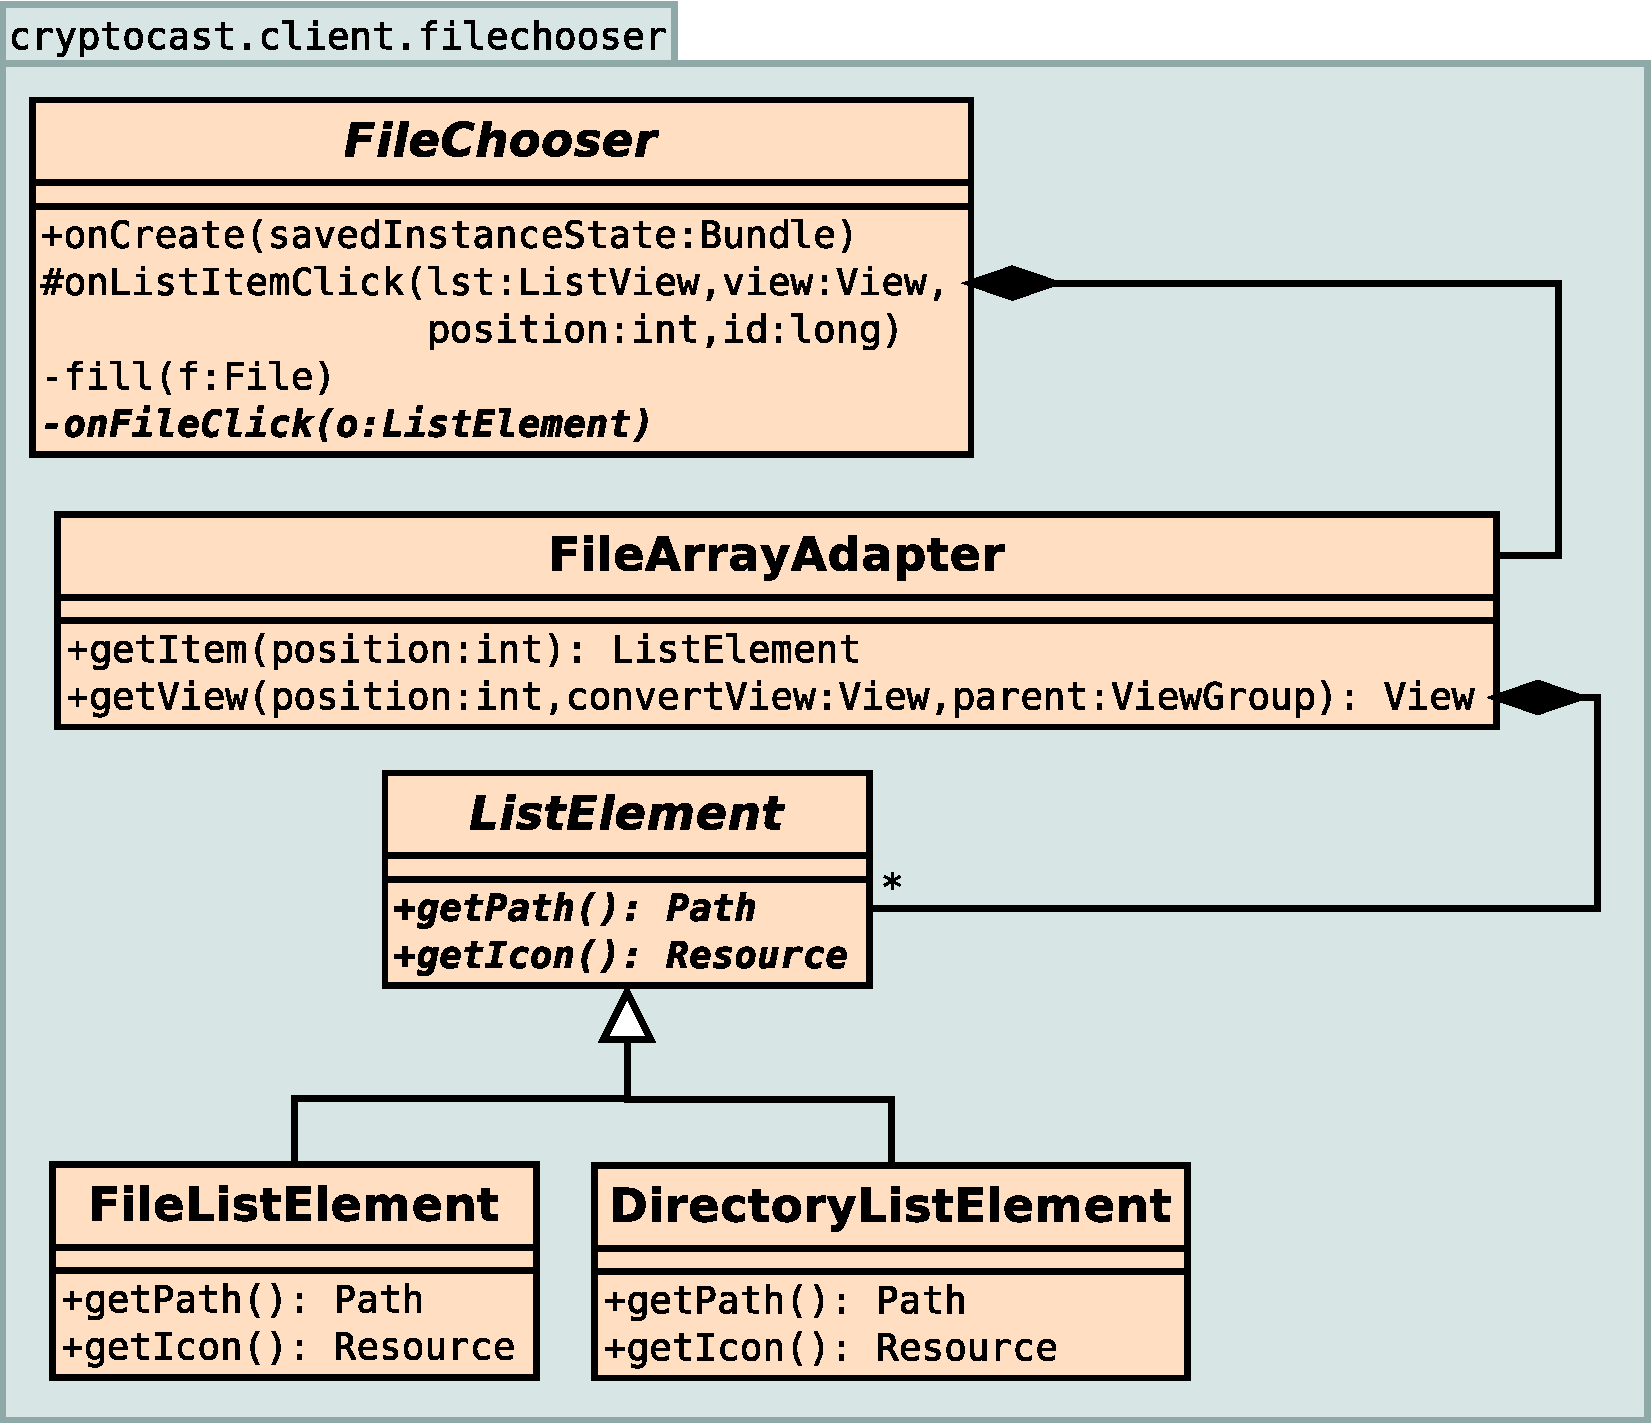
\includegraphics[width=300px]{class_diagrams/cryptocast_client_filechooser.pdf}
\end{minipage}

\subsubsection{Class \lstinline|FileListElement|}
A list element in our file chooser, representing a file. \\
\noindent\begin{minipage}[t]{5cm}
\vspace{0.3em}
\hspace*{2em}
\begin{tikzpicture}
\umlclass[]{FileListElement}{

}{
+ getPath() : Path \\ + getIcon() : Resource
}
\end{tikzpicture}
\vspace{0.3em}
\end{minipage}



\textbf{\sffamily Superclasses and Interfaces}
\begin{itemize}
\item \lstinline|cryptocast.client.filechooser.ListElement|
\end{itemize}


\textbf{\sffamily Constructors}
\begin{itemize}
\item \lstinline|public| \lstinline|FileListElement|\lstinline|(Path path)|\\ \\[-0.6em]
Creates a new instance.
\begin{itemize}
\item \lstinline|path|: The path of the file
\end{itemize}



\end{itemize}


\textbf{\sffamily Methods}
\begin{itemize}
\item \lstinline|public Path| \lstinline|getPath|\lstinline|()|\\ \\[-0.6em]
\emph{Returns:} the path of the element



\item \lstinline|public Resource| \lstinline|getIcon|\lstinline|()|\\ \\[-0.6em]
\emph{Returns:} The icon associated with this element



\end{itemize}

\subsubsection{Class \lstinline|FileArrayAdapter|}
An adapter between the ListElements and the view showing them. \\
\noindent\begin{minipage}[t]{5cm}
\vspace{0.3em}
\hspace*{2em}
\begin{tikzpicture}
\umlclass[]{FileArrayAdapter}{

}{
+ getItem(position : int) : ListElement \\ + getView(position : int, convertView : View, parent : ViewGroup) : View
}
\end{tikzpicture}
\vspace{0.3em}
\end{minipage}



\textbf{\sffamily Superclasses and Interfaces}
\begin{itemize}
\item \lstinline|android.widget.ArrayAdapter<ListElement>|
\end{itemize}


\textbf{\sffamily Constructors}
\begin{itemize}
\item \lstinline|public| \lstinline|FileArrayAdapter|\lstinline|(Context context, int textViewResourceId, List<ListElement> objects)|\\ \\[-0.6em]
Constructs a new instance with the given attributes.
\begin{itemize}
\item \lstinline|context|: The context in which this adapter is used.
\item \lstinline|textViewResourceId|: The view showing the data.
\item \lstinline|objects|: List with all elements which will be shown by the view.
\end{itemize}



\end{itemize}


\textbf{\sffamily Methods}
\begin{itemize}
\item \lstinline|public ListElement| \lstinline|getItem|\lstinline|(int position)|\\ \\[-0.6em]
\emph{Returns:} The list element at the given position in the list.
\begin{itemize}
\item \lstinline|position|: The position of the item in the list.
\end{itemize}



\item \lstinline|public View| \lstinline|getView|\lstinline|(int position, View convertView, ViewGroup parent)|\\ \\[-0.6em]
\emph{Returns:} A custom view of a list element at the given position in the list.
\begin{itemize}
\item \lstinline|position|: Position of the element in the list.
\item \lstinline|convertView|: View which should be converted.
\item \lstinline|parent|: The parent view group.
\end{itemize}



\end{itemize}

\subsubsection{Class \lstinline|FileChooser|}
A UI element that allows the user to browse the files and folders of the SD card and
 choose one file. \\
\noindent\begin{minipage}[t]{5cm}
\vspace{0.3em}
\hspace*{2em}
\begin{tikzpicture}
\umlclass[type=abstract]{FileChooser}{

}{
+ onCreate(savedInstanceState : Bundle) \\ \# onListItemClick(lst : ListView, view : View, position : int, id : long) \\ -- fill(f : File) \\ \umlvirt{-- onFileClick(o : ListElement)}
}
\end{tikzpicture}
\vspace{0.3em}
\end{minipage}



\textbf{\sffamily Superclasses and Interfaces}
\begin{itemize}
\item \lstinline|ListActivity|
\end{itemize}



\textbf{\sffamily Methods}
\begin{itemize}
\item \lstinline|public void| \lstinline|onCreate|\lstinline|(Bundle savedInstanceState)|\\ \\[-0.6em]
Initialize the instance
\begin{itemize}
\item \lstinline|savedInstanceState|: the stored state
\end{itemize}



\item \lstinline|protected void| \lstinline|onListItemClick|\lstinline|(ListView lst, View view, int position, long id)|\\ \\[-0.6em]
Handles a click onto a list item.
\begin{itemize}
\item \lstinline|lst|: The list
\item \lstinline|view|: The view
\item \lstinline|position|: The index of the list item
\item \lstinline|id|: The ID of the list item
\end{itemize}



\item \lstinline|private void| \lstinline|fill|\lstinline|(File f)| \\[-0.6em]




\item \lstinline|private abstract void| \lstinline|onFileClick|\lstinline|(ListElement o)| \\[-0.6em]




\end{itemize}

\subsubsection{Class \lstinline|DirectoryListElement|}
A list element in our file chooser, representing a directory. \\
\noindent\begin{minipage}[t]{5cm}
\vspace{0.3em}
\hspace*{2em}
\begin{tikzpicture}
\umlclass[]{DirectoryListElement}{

}{
+ getPath() : Path \\ + getIcon() : Resource
}
\end{tikzpicture}
\vspace{0.3em}
\end{minipage}



\textbf{\sffamily Superclasses and Interfaces}
\begin{itemize}
\item \lstinline|cryptocast.client.filechooser.ListElement|
\end{itemize}


\textbf{\sffamily Constructors}
\begin{itemize}
\item \lstinline|public| \lstinline|DirectoryListElement|\lstinline|(Path path)|\\ \\[-0.6em]
Creates a new instance.
\begin{itemize}
\item \lstinline|path|: The path of the directory
\end{itemize}



\end{itemize}


\textbf{\sffamily Methods}
\begin{itemize}
\item \lstinline|public Path| \lstinline|getPath|\lstinline|()|\\ \\[-0.6em]
\emph{Returns:} the path of the element



\item \lstinline|public Resource| \lstinline|getIcon|\lstinline|()|\\ \\[-0.6em]
\emph{Returns:} The icon associated with this element



\end{itemize}

\subsubsection{Interface \lstinline|ListElement|}
A list element in our file chooser, representing an element on the file system. \\
\noindent\begin{minipage}[t]{5cm}
\vspace{0.3em}
\hspace*{2em}
\begin{tikzpicture}
\umlclass[type=abstract]{ListElement}{

}{
\umlvirt{+ getPath() : Path} \\ \umlvirt{+ getIcon() : Resource}
}
\end{tikzpicture}
\vspace{0.3em}
\end{minipage}





\textbf{\sffamily Methods}
\begin{itemize}
\item \lstinline|public Path| \lstinline|getPath|\lstinline|()|\\ \\[-0.6em]
\emph{Returns:} the path of the element



\item \lstinline|public Resource| \lstinline|getIcon|\lstinline|()|\\ \\[-0.6em]
\emph{Returns:} The icon associated with this element



\end{itemize}


